\documentclass{scrartcl}

\usepackage[hidelinks]{hyperref}
\usepackage[none]{hyphenat}
\usepackage{graphicx}
\graphicspath{ {Images/} }

\title{MARKET EVALUATION AND BUSINESS CASE}
\subtitle{COMP240 - Market Evaluation}

\author{JH182233}

\begin{document}
	
	
	\maketitle
\abstract{D-Tail Entertainment is here to create a public-faced multimedia company, where we create media content in the form of Animations and Live action productions alongside game development. Additionally to create a stable, happy working environment for our employees, and a company that people want to work for. We will strive to achieving a balance of positive employee/customer satisfaction.}
	
\section{D-Tail Entertainment LTD.}

D-tail Entertainment is a multimedia company designed to create content on both video platform and the development of video games. We are looking to create the best content that we can across the board for a multitude of consumers. 

We are here to create a place where people can enjoy developing content in whichever form that they wish, whether that be creating live action shorts, game play or news coverage to making the latest D-tail game. We also want like minded passionate people to work in the best environment possible on projects that they want to make.

Our vision comes from the idea of a communal passion for games, arts and other medias, we share a drive to work with our passions and hobbies to create something that people will enjoy playing and watching. We want to live to work, rather than work to live. 

Where we are:
Currently we have a handful of ongoing projects 
\newline
Online Animated Series
Podcasts
Game Development
Content for social media (marketing)
\newline


Corporate structure:
\newline
\newline
D-Tail Animation:
Currently we are working on an online animated series, the trailer has been released and we’re in the process of completing the pilot episode.
\newline
\newline
D-Tail Games:
We are now working on MONQ, a puzzle based platformer using the mechanic of time to progress through the levels. Currently we are looking to release for May next year.
\newline
\newline
D-tail Gaming: 
Here we will be exploring the world of gaming using many formats from gameplay videos to the making of the games themselves.
\newline
\newline
D-tail Media:
We have began recording a series of podcasts that will be released weekly for entertainment/advertisement purposes.
\newline
\newline
D-Tail Productions:
D-tail Productions will be the live-action department of D-tail entertainment. 
We have recorded a few podcasts and will be working on recording some live action shorts to aid in this section of the company.


\section{Business Case}
\subsection{Objective/Problem/Opportunity}
Upon the success of this project the company will have set itself up as a reputable game developer in the eyes of the community.
The creation of a successful IP will allow further development opportunities to build upon.
The opportunity to have already worked on a project for a year, the advantages of this includes:
Overcoming issues that occur for most startups in a safe and secure environment. 
Rolling over straight into a career in industry immediately after university.

Issues to overcome could include:
Creating a product for an already established market.
Student motivation/commitment in a company can be less than satisfactory, due to their reliance on student income or not appropriate for industry.
Costs of licenses
First Time development, i.e. organisation of time and resources.
\subsection{Solution Strategy }
To address the issues stated in previous slides we will:
Perform market research to identify a gap in the market and the target audience.*
Use the agile principle for development organisation.
Treat this project as if we were in industry, by having defined working hours and contracts in place.
Turn to free software if licences are out of scope for costs.
Upon success of this project our goal will be to continue with this IP.
If this IP should fail back-up plans are in place to begin a new project immediately.

*Please refer to Market Strategy proposal for more information on this process

\subsection{SWOT Analysis}
\begin{center}
	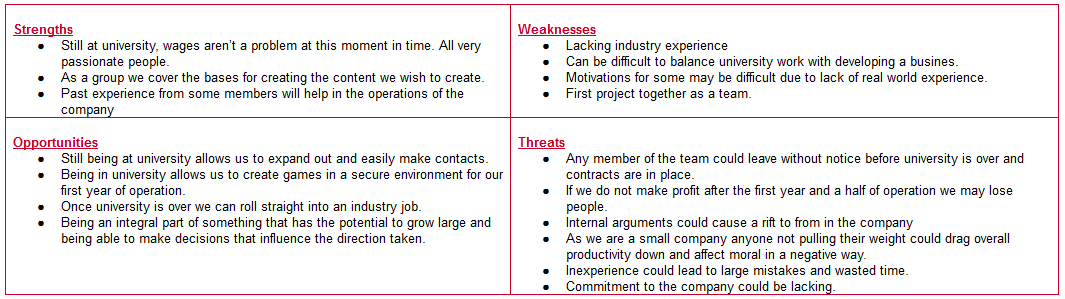
\includegraphics[scale=.5]{SWOT}	
	\newline
\end{center}


\section{Market for MONQ}
\begin{center}
	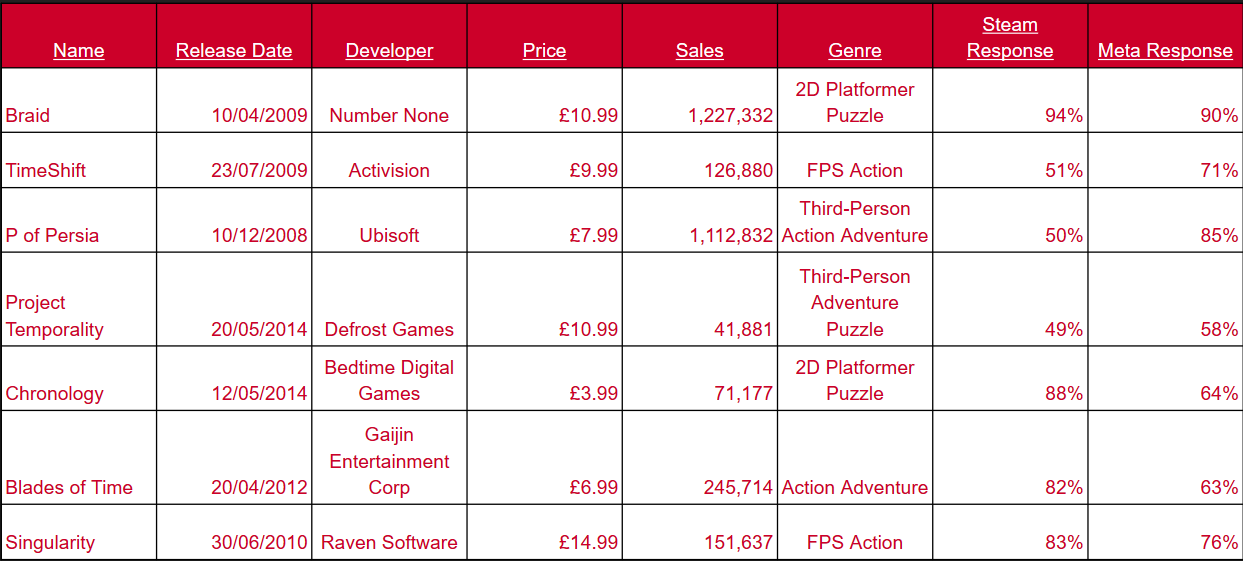
\includegraphics[scale=0.4]{ResearchChart}	
	\newline
\end{center}


The market that was looked into was for steam as that will be our primary sales platform.
Steam currently is selling 13,621 games according to SteamSpy
Looking at Time Manipulation (TM) as a mechanic only 22 are on steam and of those, Seven games where found that match MONQ.
This indicates either a small market for this type of game or a large gap in the market.
From the table there are a mixture of Indie and AAA developers that make TM games.
These games vary from 2D and 3D style games, though the highest sales achieved came from an indie company for a 2D game (Braid).
From the reviews it would seem that the 2D games tend to be received better overall than the 3D games, though the reviews are mixed so this can not carry too much weight.
Looking at the sales, TM games sell well and are considered a success on steam, ranging from £3.99-£14.99.
The last similar game to be released was back in 2014, which would indicate a current gap for TM type games.
After looking at the current market it seems to indicate that the audience we should aim for are not hardcore gamers with high end computers, but gamers that take a more relaxed approach to gaming and enjoy the puzzle element, as most of the games here share the puzzle aspect.
\newline
\newline
\newline
\newline	
When marketing you have to look at two options:
\begin{center}
	Quality of branding
	\newline
	Quantity of reach
	\newline
\end{center}
When looking at quality of branding it can be expensive as you have to go through an agency or higher a marketing specialist.
When looking at quantity of reach you can save money by going through platforms like Social media, which will get you a wide reach but:
You have to ensure the quality and delivery 
Which can lead to a negative effect on your product if done poorly.
Which you may or may not recover from.
Currently Social Media is our main focus for marketing spending a fixed budget on reaching new potential customers.

We plan on marketing through a marketing agency in the near future.
Though more research into which marketing agency will be used there are plenty of agencies in and around Cornwall.
We are primarily using steam as a selling platform as this seems to be one of the biggest platforms for small Indie companies to sell on.
Though we will be launching on itch.io for early access, to access feedback from players on how the game could be improved.
We will be offering our game from our website, but the sales on there are projected to be far less than steam, as currently the traffic through our website is not high enough.

\newpage
\section{Budgets}

The following charts show the monthly costs and income for the next year of production.
\newline
\begin{center}
	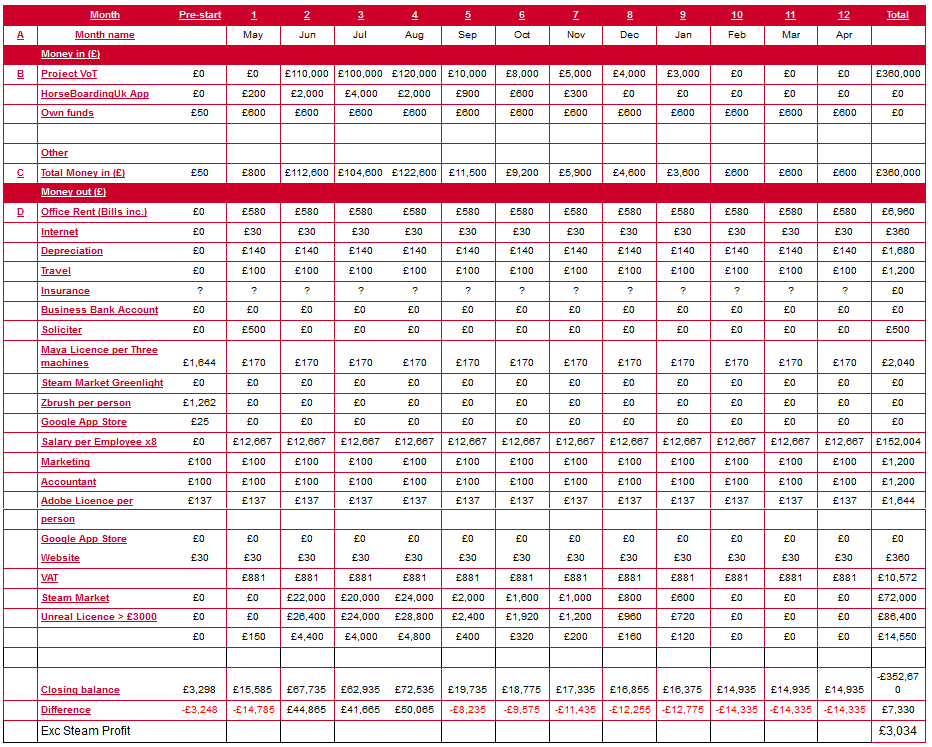
\includegraphics[scale=0.56]{CostsChart}	
	\newline
\end{center}

As you can see we must sell 33,000 units to break even. This is still lower than the worst selling game of similar mechanics on steam.
From play-testing it has been suggested to us that we sell the game for no less than Ten Pounds per copy, this is the price that will be asked for on the marketplace.
\newline
\begin{center}
	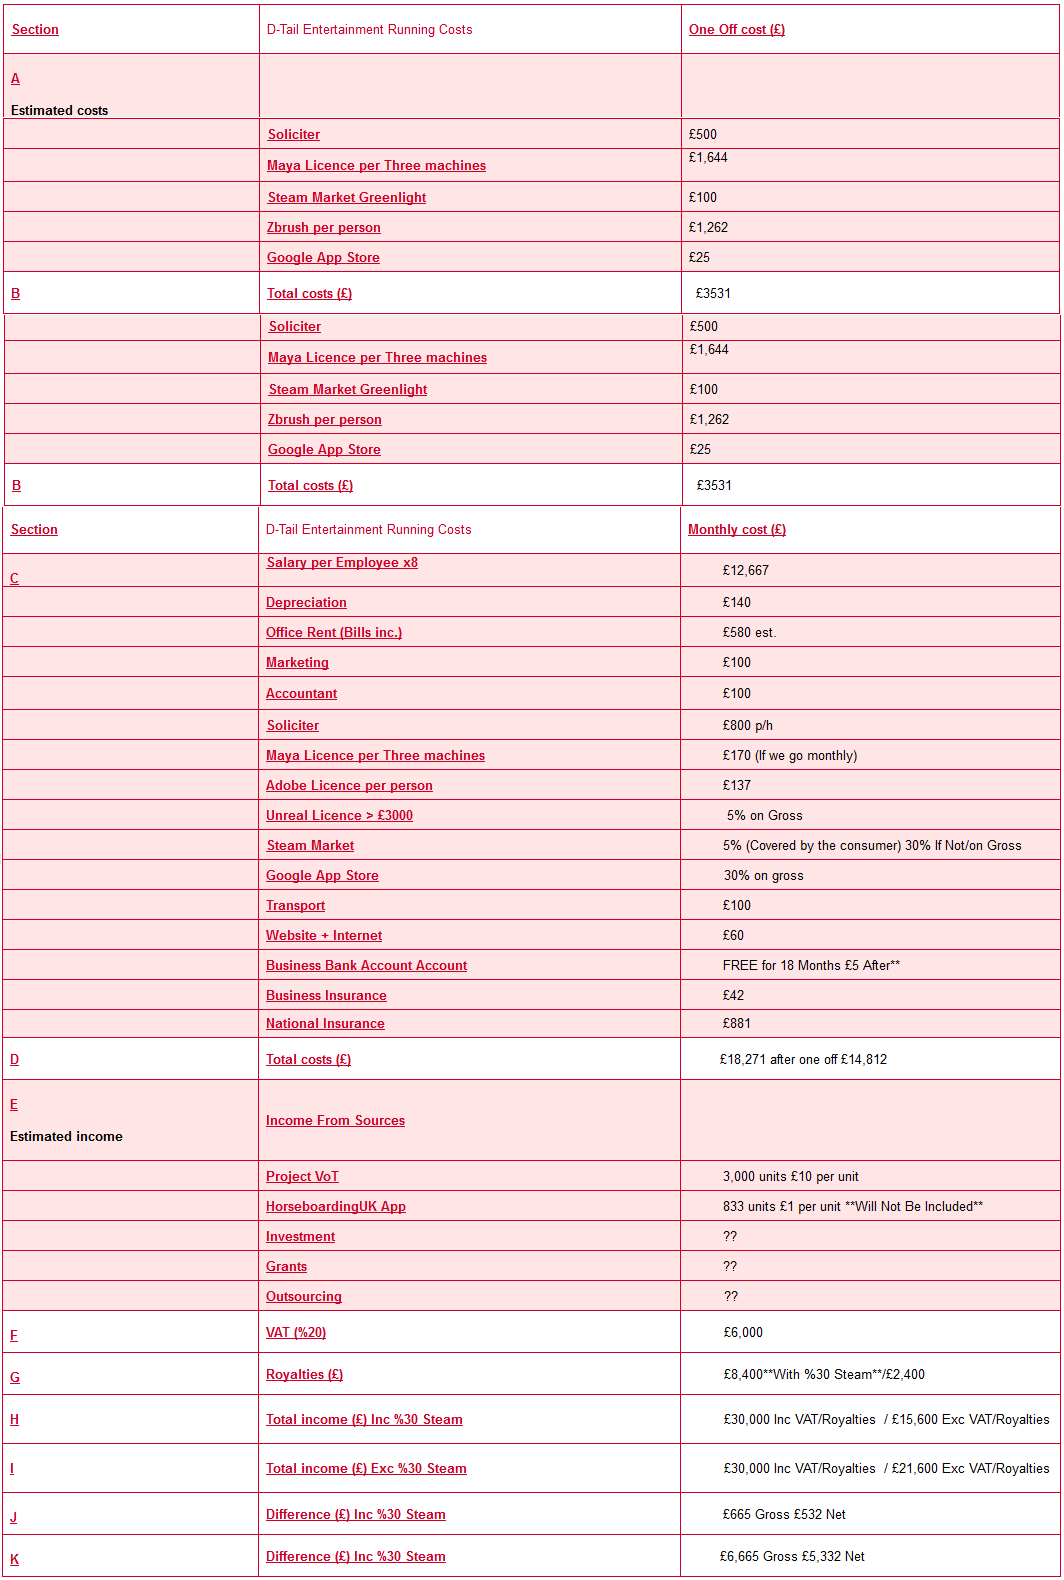
\includegraphics[scale=0.56]{CostsChartLong}
\end{center}
	
											
	\bibliographystyle{apalike}
	\bibliography{Journal}
											
\end{document}